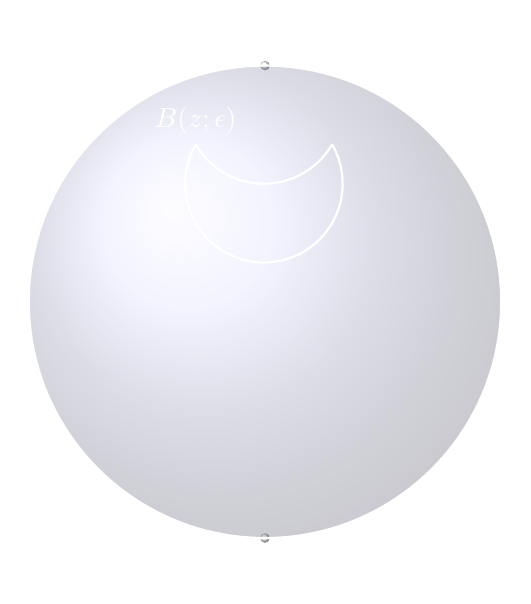
\begin{tikzpicture}[scale=2]

  % radius of the sphere
  \def\r{1.5}

  % coordinates
  \coordinate (O) at (0,0,0);
  \coordinate (N) at (0,\r,0);
  \coordinate (S) at (0,-\r,0);

	\shade[ball color=white] (N) circle (0.03);
  \shade[ball color=white] (S) circle (0.03);
  \node[above right, white] at (N) {$N$};
  \node[below right, white] at (S) {$S$};

  % Draw a translucent sphere (Bloch-sphere-style)
	\shade[ball color=blue!20, opacity=0.3] (0,0) circle (\r);

  % Equator (great circle in xy-plane)
  \draw[thick, white] (O) circle (\r);

	\def\R{0.5}      % main circle radius
  \def\alpha{30}   % half-angle of cavity

	\coordinate (C) at (-0.5 + \alpha * 0.002, 1);	% center of a circle

	\shade[ball color=white] (C) circle (0.00) node[above, white] {$B(z;\epsilon)$};

  % main circle minus top
  \draw[thick, white] (C) arc[start angle=180+\alpha, end angle=360-\alpha, radius=\R];

  \draw[thick, white] (C) arc[start angle=180-\alpha, end angle=360+\alpha, radius=\R];

\end{tikzpicture}

